
\ifx\isEmbedded\undefined
\pdfobjcompresslevel 0
\documentclass[a4paper, 12pt]{report}


%
%%\usepackage{comment} % Permet de compiler sans les figures et sans les tables
%%\excludecomment{figure}
%%\let\endfigure\relax
%%\excludecomment{table}
%%\let\endtable\relax

%\usepackage{refcheck} %permet de voir les refs du bib non cit�es

\setlength{\parindent}{0pt} %get rid of indentation in the article
\usepackage{etoolbox} % prevent a Patching '\begin' failed! see https://tex.stackexchange.com/questions/128938/package-etoolbox-warning-patching-begin-failed
%\usepackage{natbib} % pour bibtex \citep (parenthetical) et \citet (textual) (sinon seul \cite marche) a loader avant babel
\usepackage[semicolon,round,sort&compress,sectionbib]{natbib}  %
\usepackage{chapterbib}      
\usepackage[english, french]{babel} %Fran�ais à loader avant caption
\usepackage[T1]{fontenc}

  \usepackage{adjustbox}
\usepackage[affil-it]{authblk} %for affiliation
\usepackage{afterpage} % To include blanck page with command \afterpage{\blankpage}
\usepackage{appendix}

\usepackage{array} %pour les tableaux
\usepackage{amsmath, amssymb} %american mathematical society math style and symbols (amssymb)
\usepackage{amsthm}
\usepackage{blindtext}
\usepackage{booktabs}
\usepackage{breqn} % allow to use dmath environment (automatic break for equations, etc) 
\usepackage{caption} % Needed to jump line in figures titles (caption).
%\usepackage{commath} sais pas pourquoi �a marche pas si je charge �a plante !

\usepackage{dirtytalk} % quote stuff with \say{the text to quote}
\usepackage{empheq} %
\usepackage[official]{eurosym}  %type \euro{} to print a euro
\usepackage{float} % for firgure placement with H option
\usepackage{fancybox}

  \usepackage[top=2cm, bottom=2cm, left=2.5cm, right=2.5cm]{geometry}
  \usepackage[top=2cm, bottom=2cm, left=2.5cm, right=2.5cm]{geometry}
\usepackage{graphicx} %pour ins�rer des images.
 \usepackage[hyperindex=true,
 		     colorlinks=true, 
		     urlcolor=blue,
		     citecolor    = blue, %Couleur des citations (biblio)
    		     linkcolor    = blue, %Couleur des équations. Apparemment, cela sert aussi pour théoreme, Lemme...
 					 ]{hyperref} %permet de mettre des hyper liens (le package url le fait tout seul ? la base)

\usepackage{import}					 



\usepackage{pdflscape}
\usepackage{pdfpages} %allow to select which pdf pages to compile \includepdf[pages={12-15,23,45-49}]{main.pdf} 
\usepackage{spverbatim}
\usepackage{lmodern}%change un peu les lettres pour un truc plus cool, marche peut �tre un peu mieux avec les accents v�rifier � l'occaz
\usepackage{mathrsfs} % allows $\mathscr{ABC}$ to work
\usepackage{setspace} % permet de d�terminer une largeur d'interligne
\usepackage{tikz} % draw graphs
\usetikzlibrary{trees,shapes,snakes}
  \usepackage{subcaption} % to use with subfigures
\usepackage{skull}
\usepackage{url}
\usepackage{verbatim} %Pour ins�rer du code informatique

\usepackage{fancyvrb}
\usepackage{fvextra}

\usepackage{array} %one of the two needed to use thead to break line in tabular
\usepackage{makecell} %one of the two needed to use thead to break line in tabular

\DeclareUnicodeCharacter{20AC}{\euro{}}
\DeclareUnicodeCharacter{2212}{-}
\DeclareUnicodeCharacter{300}{`}
\DeclareUnicodeCharacter{301}{'}

  \newcommand{\hdrule}{\midrule[\heavyrulewidth]}

\newsavebox{\mybox}

\newcommand{\raisedshadowbox}[1]{%
\sbox\mybox{\shadowbox{#1}}%
\raisebox{-0.5\ht\mybox-0.5\shadowsize+0.6ex}{\usebox\mybox}%
}
%%%%%
\providecommand{\tightlist}{%
  \setlength{\itemsep}{0pt}\setlength{\parskip}{0pt}}


\bibliographystyle{chicagoa}


%%%%%%%%%%%%%%%%
%%%Fin biblio %%%%%%%%



%%%%Elispse in tables%%%%%%
\usepackage{tikz}
\usetikzlibrary{fit,shapes.misc}
\newcommand\marktopleft[1]{%
    \tikz[overlay,remember picture] 
        \node (marker-#1-a) at (0,-1ex) {};%
}
\newcommand\markElipseBottomright[1]{%
    \tikz[overlay,remember picture] 
        \node (marker-#1-b) at (0.2,0.3) {};%
    \tikz[overlay,remember picture,thick,dashed,inner sep=3pt]
        \node[draw, ellipse,fit=(marker-#1-a.center) (marker-#1-b.center)] {};%
}
%%%%End Elispse in tables%%%%%%






%%%%Squares in tables%%%%%%
\newcommand\markRectangletopleft[1]{%
    \tikz[overlay,remember picture] 
        \node (marker-#1-a) at (0,1.5ex) {};%
}
\newcommand\markRectanglebottomright[1]{%
    \tikz[overlay,remember picture] 
        \node (marker-#1-b) at (0,0) {};%
    \tikz[overlay,remember picture,thick,dashed,inner sep=3pt]
        \node[draw,rounded rectangle,fit=(marker-#1-a.center) (marker-#1-b.center)] {};%
}
%%%%Squares Circles in tables%%%%%%


\newcommand\blankpage{%
    \null
    \thispagestyle{empty}%
    \addtocounter{page}{-1}%
    \newpage}




\DeclareMathOperator\erf{erf}


\providecommand{\U}[1]{\protect\rule{.1in}{.1in}}
%EndMSIPreambleData
\newtheorem{theorem}{Theorem}
\newtheorem{acknowledgement}[theorem]{Acknowledgement}
\newtheorem{algorithm}[theorem]{Algorithm}
\newtheorem{axiom}[theorem]{Axiom}
\newtheorem{case}[theorem]{Case}
\newtheorem{claim}[theorem]{Claim}
\newtheorem{conclusion}[theorem]{Conclusion}
%\newtheorem{condition}[theorem]{Condition}
\newtheorem{conjecture}[theorem]{Conjecture}
\newtheorem{corollary}[theorem]{Corollary}
\newtheorem{criterion}[theorem]{Criterion}
\newtheorem{definition}[theorem]{Definition}
\newtheorem{example}[theorem]{Example}
\newtheorem{exercise}[theorem]{Exercise}
\newtheorem{lemma}[theorem]{Lemma}
\newtheorem{notation}[theorem]{Notation}
\newtheorem{problem}[theorem]{Problem}
\newtheorem{proposition}[theorem]{Proposition}
\newtheorem{remark}[theorem]{Remark}
\newtheorem{solution}[theorem]{Solution}
\newtheorem{summary}[theorem]{Summary}
%\newenvironment{proof}[1][Proof]{\noindent\textbf{#1.} }{\ \rule{0.5em}{0.5em}}



\usepackage{fancyhdr}

\usepackage{minitoc} % table of contents should be loaded after hyperef and other packages
\usepackage{silence}


%%%%% Mute minitoc warnings see https://tex.stackexchange.com/questions/166910/what-are-these-warnings-for-minitoc-package
\WarningFilter{minitoc(hints)}{W0023}
\WarningFilter{minitoc(hints)}{W0024}
\WarningFilter{minitoc(hints)}{W0028}
\WarningFilter{minitoc(hints)}{W0030}
\WarningFilter{blindtext}{} % this takes care of the `blindtext` messages

\usepackage{grffile}

\graphicspath{{}}

\frenchbsetup{ShowOptions} 

\Urlmuskip=0mu  plus 10mu  %Solver Overfull \hbox for url links (see https://tex.stackexchange.com/questions/339682/how-to-really-solve-the-problem-of-underfull-hbox-when-typesetting-url-in-f)

\begin{document}

\selectlanguage{french} 

\else \fi

%%%%%%%%%%%%%%%%%%%%%%%%%%%%%%%%%%%%%%%%%%%%%%

\chapter*{Remerciements}

\addcontentsline{toc}{chapter}{Remerciements}


Cette thèse a commencé par une passion pour l’économie, et pour l’économie publique. Je remercie Bruno Decreuse pour le cours d’introduction à l’économie, et les conseils de lecture donnés lors du cours. L’aspect ludique du cours et la qualité de l’enseignement sont les raisons premières qui ont je pense fait naitre en moi l’envie de faire de la recherche en économie. 


\medskip


Je  remercie l’équipe d’Étalab qui m’a accueilli lors de mon stage de Master II , et particulièrement Emmanuel Raviart, et Christophe Benz qui ont eu la patience de me fournir une première éducation sur des outils essentiels tels que Python et git. 


Un immense merci à Mahdi Ben Jelloul, le papa d’OpenFisca, qui m’a suivit, soutenu et aidé tout au long de ma thèse,  et sans qui les résultats du premier chapitre de cette thèse n’auraient jamais vu le jour.


\medskip
Merci également à tout les doctorants de l’AMSE dont les conversations riches et animées,  les conseils, et soutiens ont permis d’égailler les journées de travail pas toujours faciles. 
Je pense à ce qui étaient déjà en doctorat avant que cette thèse ne commence. Nicolas Abad pour avoir été un ami et encouragé à faire de la recherche dès ma licence 3. Sébastien Gharbi pour les discussions philosophiques fleuves à l’époque où je souhaitais faire de l’économie normative. Mais aussi à Lise Clain, Bilel Sanhaji, Kadija Charni, Régis Sawadogo, Ugo Boletta, Florent Dubois, à Pauline Morault, Thomas Chouffard, Clémentine Sadania pour les sorties escalades, Joao Varendas, et Damien Sans. Paul Maarek pour les conseils.


Il y a eu aussi les boursiers de 4 ème année, Laurine Martinoty merci pour les conversations, échanges de livres et conseils de lecture (surtout Yourcenar), et l’hébergement à Pantin. Yannick Dupraz pour m’avoir fait découvrir booktab et les verres à Sartrouville, merci.


Mais également les doctorants de ma génération, merci à Lara Vivian, Audrey Étienne, Ilia Gouaref, Victorien Barbet, François Reynaud. Merci à Charles O’Donnel pour les nombreux hébergements sur Paris, les couscous à Marseille et sa bonne humeur constante. Merci à Vera Danilina, meilleur co-bureau du monde pour ses conseils, son amitié, et sa rigueur à toute épreuve.


Quant au doctorants  ayant commencé après, merci à Tangy le Fur pour ses discussions toujours caustiques, Vernon Subutex, les bières et le manouche. Merci à Edwin Fourrier pour le rire qui réveille et les séances d’Altissimo. Merci à Armel Ngami et le Bois Chéri, Stéphane Benveniste, Morgan Raux, Laura  Sénécal, Florian Guibelin, Pavel Molchanov, Alberto Prati, Edward Levavasseur, Ulises Genis, Loann Desboulets pour tous les conseils en économétrie, Anushka Chawla, Kathia Bahloul, Ulrich Nguemdjo-Kamguem,Océane
Piétri, Rémi Vives, et Samuel Kembou Nzale.

\medskip

D’autres doctorants que ceux de l’AMSE on été présents durant cette thèse. Une gratitude infinie à Malka Guillot, pour sa passion, ses encouragements, conseils et aides du début à la toute fin de cette thèse. Merci à Erwan Moussault pour m’avoir intégré à Cergy, ses conseils, ses invitations aux soirées. Merci à Adrien Fabre pour avoir égaillé mon stage de Master II, les conversations et conseils mais également d’avoir libéré ce qui était prisonnier dans la forteresse.  Merci aussi aux doctorants en sociologie du centre Norbert Elias, et en particulier Edgard et Manon.

\medskip

Merci au personnel administratif, avec une pensée émue pour Carole Maillard. Merci à Bernadette Vouriot d’avoir toujours su gérer ma phobie administrative avec bienveillance. Merci à Laurence Bouvard pour le soutien, les données, et la sympathie. Merci également à Marine Boléa et Gregory Cornu de joyeux drilles  toujours bienveillants.
Je remercie aussi, Corinne Michaud, Aziza Sikar, Yves Doazan, Agnès Chaussonnaud, Gérald Chapuis, Elisabeth Barthélemy , et Kaina Tighilt.

\medskip


Merci également à tout les chercheurs séniors pour tous leurs conseils et soutiens divers, je pense notamment à Laurence Jacquet,  Michel Lubrano, Etienne Lehmann, Tanguy van Ypersele, Nicolas Gravel, Fabian Gouret, Antonin Mace, Sebastian Bervoets, Frédéric Dufourt,  Bruno Decreuse, Jernej Copic pour sa sympathie, et Pierre Pestieau, pour m’avoir informé sur l’existence des travaux de Vickrey sur la temporalité de l’impôt.


\medskip


Merci également à Stephen Bazen et Xavier Joutard, les directeurs du magistère ingénieur économiste à l’époque ou j’étais dans cette formation, pour leurs conseils durant cette thèse. Merci aux anciens du magistère, ça a été une aventure ! Merci  Khalid Maman-Waziri,  Majda Benzidia, Edmond Noack pour tous les verres au petit Nice, Mathieu Donneti pour notre projet de finance sur les queues épaisses rédigé sous Latex (et probablement le plus beau document que j’ai produit à ce jour).





\medskip


Merci à Ewen Gallic et Pierre Michel pour leur sympathie, que leur début de carrière de MCF soit des plus fructueuse. Merci à Pierre Pecher.

\medskip


Merci à ceux qui, lorsque j’étais prêt à abandonner, ont par leurs mots, permis de faire en sorte que ce ne soit pas le cas, je pense en particulier à Majda Benzidia, Marc Sangnier, et Malka Guillot.

\medskip


Merci aux amis qui sont restés présents toutes ces années, Florian, Anthony, Antoine, Victor, Sarah, Olivia, Camille  Mamie et Camille V, Geoffrey, Nina, Maxime, Noémie,  Nicolas M, Sylvain Natcho, Jane, Jade, Fanny Loutre, Estelle, et Marine. 


Merci à tous les colocs, avec un pensée particulière pour Rébecca, Ludo Chouchou, Laurence, Youri,  Thomas, Rémi, Carole, Aurélie pas chat et Manu, Bérengère, et Kevin.


\medskip


Merci à ma famille, et en particulier merci à mes parents qui ont été d’un soutient constant.


\medskip


Merci aux nombreuses personnes, qu’elles soient Richard Stallman, ou inconnues qui ont contribué au libre ces  quarante dernière années, --ce qui je crois sera le plus grand bien public du XXIe siècle — pour avoir permit l’émergence de l’ensemble des outils qui ont servi à la réalisation de cette thèse.


\medskip


Je remercie également les membres du jury d’avoir accepté de lire et juger cette thèse.  Et pour finir, "last but not least", merci à mes directeurs de thèse Olivier Bargain et Alain Trannoy d’avoir tenu bon toutes ces années (je ne leur ai pas rendu la tâche facile) et sans qui cette thèse n’aurait pas été possible.


 
%%%%%%%%%%%%%%%%%%%%%%%%%%%%%%%%%%%%%%%%%%%%%%


\ifx\isDoubleEmbedded\undefined
\newpage
%\bibliography{../../Biblio/biblio-rapport}
\end{document}
\else \fi


